\newpage
\section{Lo Strato di Rete IP}
Lo \textbf{\textcolor{purple}{strato di rete IP}} dello stack protocollare TCP/IP fornisce un meccanismo per la consegna di datagrammi tra host.
Viene sfruttato da tutti i protocolli del livello di trasporto e utilizza meccanisi del livello di collegamento.
Le peculiarità del livello di rete IP (anche e soprattutto rispetto ai livelli superiori) sono:
\begin{itemize}
    \item La presenza non solo negli host mittente e destinatario ma anche nei router;
    \item Interconnessione di reti eterogenee, questo offre un’astrazione che consente a host e reti eterogenee di funzionare dal punto di vista logico come una singola rete;
    \item Implementazione di un numero di funzionalità limitato.
    \item Punto nevralgico nello stack protocollare TCP/IP. Questo infatti rappresenta il punto di connessione tra la parte superiore e inferiore dello stack, permettendo un evoluzione indipendente dei protocolli. 
\end{itemize}
\newblock
I passaggi di funzionamento sono i seguenti:
\begin{enumerate}
    \item L’entità a livello di rete riceve i segmenti dal livello di trasporto nell’host mittente, e incapsula i segmenti in datagrammi;
    \item I datagrammi sono inoltrati al prossimo nodo (host o router);
    \item Il router esamina i campi intestazione in tutti i datagrammi IP che lo attraversano e li inoltra da un collegamento in ingresso ad un collegamento in uscita;
    \item Sul lato destinatario, consegna i segmenti al livello di trasporto.
\end{enumerate}

\subsection{Servizi}
IP è un protocollo di tipo:
\begin{itemize}
    \item \textcolor{purple}{Connection-Less:} non c’è circuito virtuale né fisico fra i due sistemi terminali a livello IP;
    \item \textcolor{purple}{Best Offert:} non c’è garanzia che i pacchetti vengano ricevuti nell’ordine in cui sono stati inviati, ne tanto meno ricevuti;
\end{itemize}
IP in generale non è affidabile e non presenta inoltre meccanismi di \textcolor{purple}{QoS} (Quality of Service) sul tempo di consegna dei datagrammi e sul controllo di flusso.
\newpage
Nonostante questo IP offre quali:
\begin{itemize}
    \item \textcolor{purple}{Suddivisione in pacchetti:} modello datagram senza connessione per la consegna dei dati;
    \item \textcolor{purple}{Forwarding o Inoltro:} trasferimento del pacchetto sull’appropriato collegamento di uscita;
    \begin{figure}[h]
        \centering
        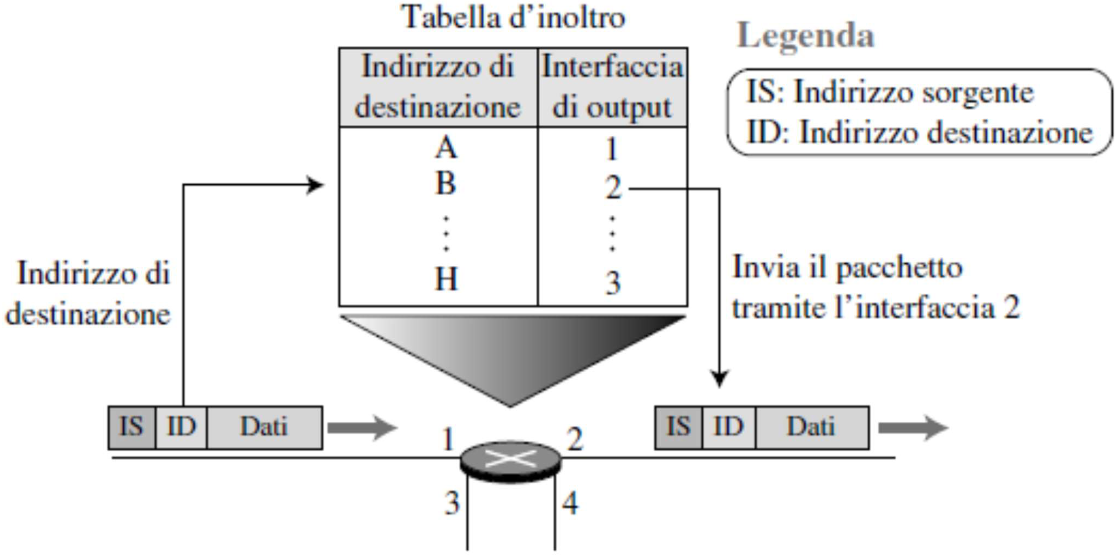
\includegraphics[scale=0.28]{Immagini/IndirizzamentoIP.png}
    \end{figure}
    \item \textcolor{purple}{Routing o Instradamento:} processo decisionale di scelta del percorso verso una destinazione (algoritmi di instradamento o routing);
    \begin{figure}[h]
        \centering
        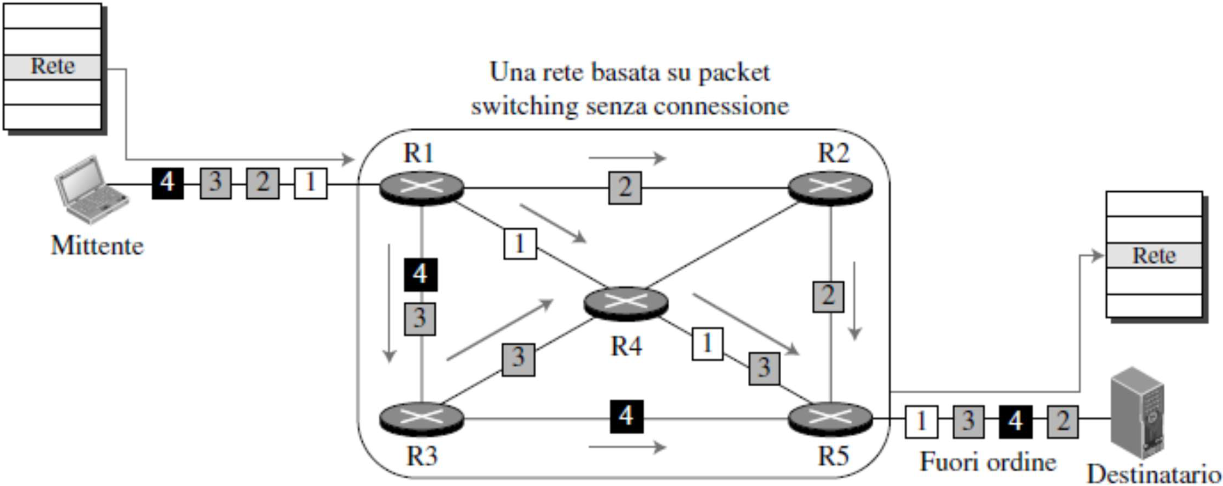
\includegraphics[scale=0.28]{Immagini/ForwardingIP.png}
    \end{figure}
    \item \textcolor{purple}{Multeplexint/Demultiplexing:} anche in questo caso sono presenti meccanismi di multiplexing e di Demultiplexing come già visto nel livello di trasporto.
\end{itemize}

\newpage
\subsection{Formato Datagramma IP}
\begin{figure}[h]
    \centering
    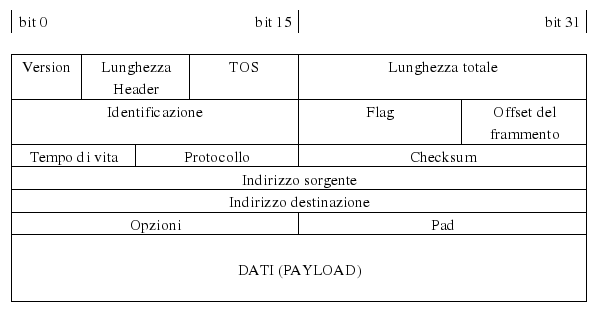
\includegraphics[scale=0.5]{Immagini/IPFormatoDatagramma.png}
    \caption{Formato Datagramma IP.}
\end{figure}

La semantica dei vari capi è la seguente:
\begin{itemize}
    \item \textcolor{purple}{Versione:} specifica la versione di IP usata (attualmente IPv4 o IPv6); 
    \item \textcolor{purple}{Lunghezza Header:} lunghezza dell'header espressa in parole da 32 bit.
    \item \textcolor{purple}{TOS:} (Tipo di Servizio) serve per “colorare” il datagramma IP (basso ritardo, affidabilità, ecc...). 
    \\Inizialmente Type of Service, poi:
        \begin{itemize}
            \item 6 bit per \textcolor{purple}{Differentiated Services}, i pacchetti vengono marcati in base alla classe di servizio (telefonata, controllo, multimedia streaming, dati a bassa priorità) in quanto i router utilizzano per ciascuna tipologia differenti politiche di accodamento;
            \item 2 bit per \textcolor{purple}{Explicit Congestion Notification} (ECN), supporto a livello rete e trasporto per la notifica di eventi di congestione.
        \end{itemize}
    \item \textcolor{purple}{Lunghezza del datagramma:} è la lunghezza di tutto il datagramma in byte, header incluso. (teoricamente la dimensione massima sarebbe 65535 byte, ma nella pratica è 1500);
    \item \textcolor{purple}{Identificatore, Flag e Offset:} sono campi per la gestione della frammentazione che vedremo in dettaglio successivamente;
    \item \textcolor{purple}{Tempo di vita:} ad ogni passaggio da un router viene decrementato, quando raggiunge lo zero viene scartato. Assicura che eventuali percorsi ad anello non provochino traffico perpetuo nella rete. (Il valore iniziale dipende dal SO: 30, 64, 128, 255);
    \item \textcolor{purple}{Protocollo:} indica all’host destinatario a quale protocollo dello strato superiore inoltrare i dati;
    \item \textcolor{purple}{Checksum dell'intestazione:} viene calcolato il checksum della sola intestazione (ponendo questo campo pari a zero) ad ogni router (il TTL cambia ad ogni hop);
    \item \textcolor{purple}{Indirizzo sorgente/destinazione:} indirizzo IP rispettivamente del mittente e del destinatario;
    \item \textcolor{purple}{Opzioni:} campo usato sporaticamente di dimensione massima di 40 byte.
    \item \textcolor{purple}{Payload:} dati effettivamente trasportati dal datagramma IP.
\end{itemize}

Una osservazione non banale è quella di capire perchè i protocolli di trasporto TCP e UDP (opzionalmente) si preoccupano di verificare l'integrità delle informazioni anche se già IP utilizza una checksum.
Per iniziare IP non esegue la checksum sui dati, ma solamente sull' header. Inoltre la checksum di TCP e UDP viene eseguita solamente sui punti terminali della connessione mentre quella di IP viene eseguita per ogni nodo del trasferimento.

\subsection{Frammentazione}
\begin{definition}
    L'\textbf{\textcolor{purple}{MTU}} (Maximum Transfer Unit) è la quantità massima di dati trasportata dal protocollo di collegamento in un frame.
\end{definition}
Questo valore varia tra una tecnologia e l'altra (es, Ethernet 1500, ATM 576, FDDI 4500...).
\\Il meccanismo di frammentazione è quel processo nel quale, dato un datagramma IP che supera in dimensione l'MTU del collegamento sul quale deve essere inoltrato, questo viene suddiviso in due o più datagrammi di dimensione inferiore, detti \textcolor{purple}{frame}.
L'operazione di riassemblaggio di questi frame viene eseguita dall' entità di rete nel sistema terminale. 
Se durante tutto questo processo anche un solo frame viene perso, viene buttato via l'intero datagramma.
\\Essendo ogni frame un datagramma IP a tutti gli effetti, questi vengono trasmessi indipendentemente dagli altri.
Inoltre, come accade per i segmenti TCP, i frame possono essere consegnati fuori ordine e per ricostruire il datagramma originale vengono utilizzati i sequenti flag dell' header:
\begin{itemize}
    \item \textcolor{purple}{Identificatore:} è associato al datagramma dall’host sorgente treamite IP sorgente e IP destinazione, identifica quel datagramma in un intervallo di tempo ragionevolmente lungo. I frame di quel datagramma mantengono il valore di questo campo in modo tale che il destinatario riconosca i frame che vanno assemblati insieme;
    \item \textcolor{purple}{Offset:} indica la posizione relativa del primo byte del frame rispetto al datagramma originale. Il primo frame avrà offset 0 e ogli frame avrà una dimensione del paylaod che è multipla di 8; 
    \item \textcolor{purple}{Flag,} serve per indicare l'ultimo frame:
        \begin{itemize}
            \item il bit 0 è riservato
            \item il bit 1 detto \textcolor{blue}{do not fragment} vale:
                \begin{itemize}
                    \item 0, se il pacchetto può essere frammentato;
                    \item 1, se il pacchetto non deve essere frammentato.
                \end{itemize}
            \item il bit 2 detto \textcolor{blue}{more fragments} vale:
                \begin{itemize}
                    \item 0, se il frame è l'ultimo del datagramma originale;
                    \item 1, altrimenti.
                \end{itemize}
        \end{itemize}
\end{itemize}

\begin{figure}[h]
    \centering
    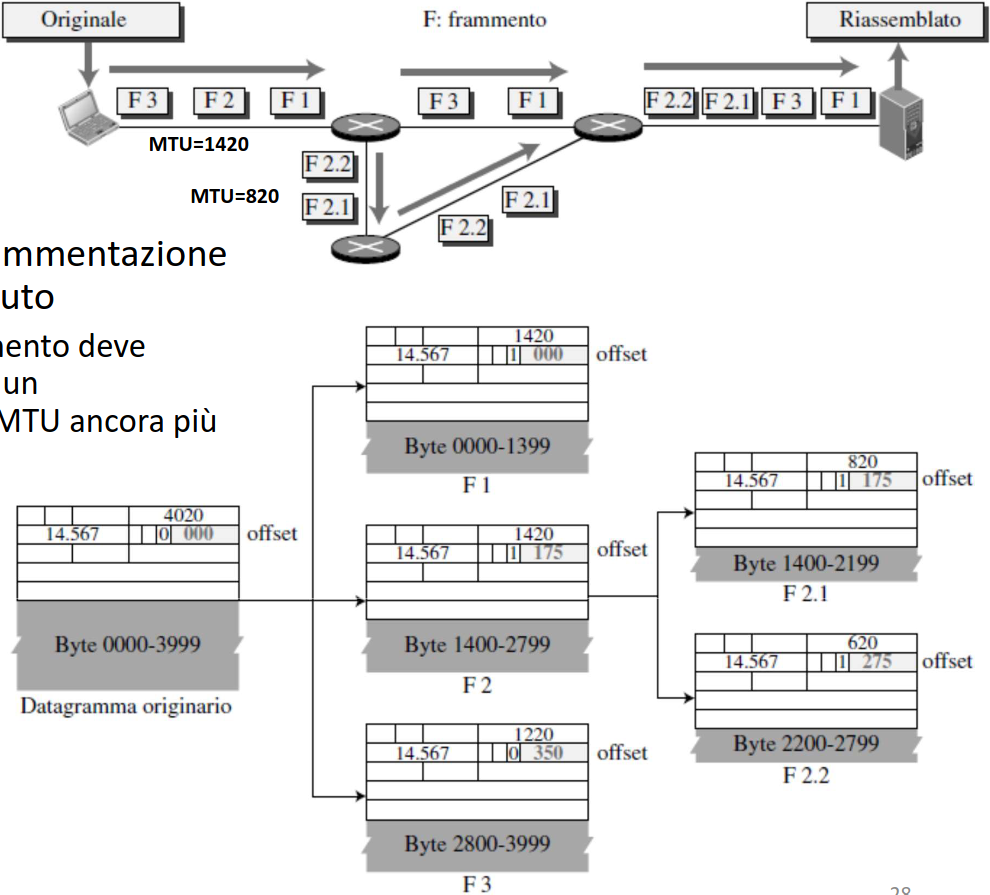
\includegraphics[scale=0.33]{Immagini/FrammentazioneIP.png}
    \caption{Esempio di frammentazione.}
\end{figure}

Come detto anche precedentemente, essendo ogni frame un datagramma IP a tutti gli effetti, questi possonon essere frammentati a loro volta.
\newpage 
In generale però il processo di frammentazione è un operazione delicata. Sono necessarie risorse in ogni nodo della rete, ritardi di eleboarzione ed è presente il rischio di perdere un intero datagramma per la mancanza di un singolo frame (anche non di primo livello).
Si decide perciò di non frammentare e in particolare questo tipo di operazione non è supportata da IPv6.

\subsection{Indirizzamento IP}
Ogni host è connesso ad Internet attraverso un'interfaccia di rete, che è il confine fra l'host ed il collegamento su cui vengono inviati i datagrammi.
Ad ogni interfaccia è assegnato un indirizzo IP \textcolor{purple}{univoco} e i router devono necessariamente essere connessi ad almeno due interfaccie.
\\Gli indirizzi IP sono costituiti da 32 bit rappresentati in notazione decimale puntata \textcolor{blue}{a.b.c.d} con a,b,c e d singoli byte.
\\Gli indirizzi degli host sono divisi in due parti:
\begin{itemize}
    \item \textcolor{purple}{Network ID:} che identifica una certa rete;
    \item \textcolor{purple}{Host ID:} che identifica un certo host in una specifica rete.
\end{itemize}

Per identificare il numero n di bit in un indirizzo che specificano la rete si utilizzano due strategie differente dette \textcolor{purple}{Classfull} e \textcolor{purple}{Classless Addresing}

\subsubsection{Classful Addresing}
Gli indirizzi vengono suddivisi in base al al prefisso dell'indirizzo in classi dalle A alla E:
\begin{itemize}
    \item \textcolor{purple}{Classe A:} 7 bit per 128 reti IP da 16 milioni di host, con indirizzi da 0.0.0.0 a 127.255.255.255;
    \item \textcolor{purple}{Classe B:} 14 bit per ca. 16000 reti IP da ca. 64000 host, con indirizzi da 128.0.0.0 a 191.255.255.255;
    \item \textcolor{purple}{Classe C:} 21 bit per ca. 2 milioni di reti IP da 256 host, con indirizzi da 192.0.0.0 a 223.255.255.255;
    \item \textcolor{purple}{Classe D:} riservata a multicast con indirizzi da 224.0.0.0 a 239.255.255.255;
    \item \textcolor{purple}{Classe E:} riservata per usi di futuri/ricerca con indirizzi da 240.0.0.0 a 255.255.255.
\end{itemize}

\begin{figure}[h]
    \centering
    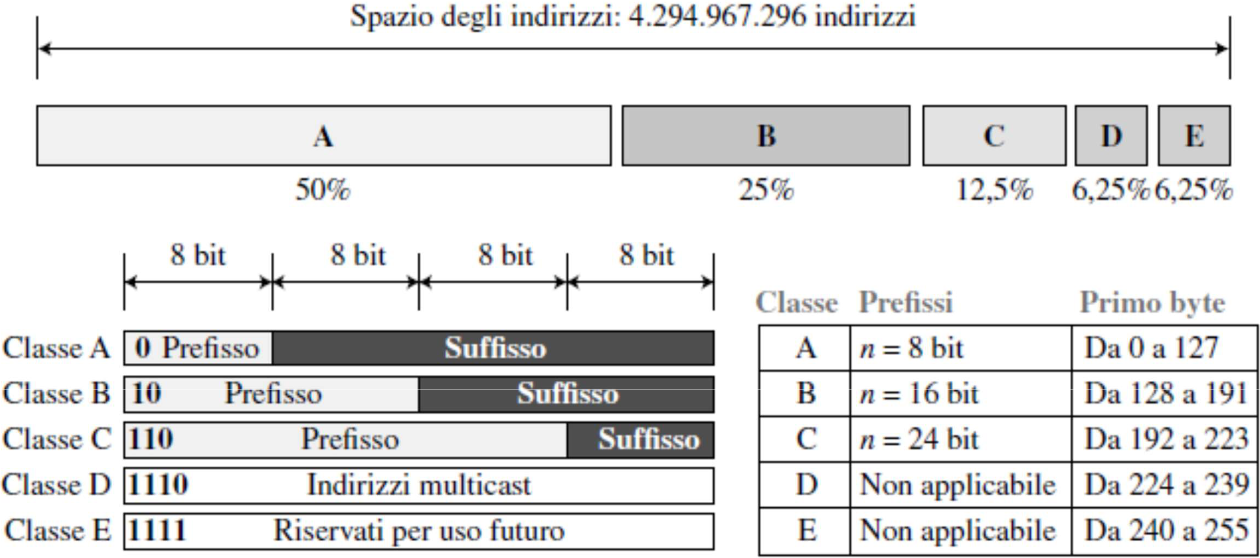
\includegraphics[scale=0.27]{Immagini/ClassfulAddressingIP.png}
    \caption{Classful addressing.}
\end{figure}

Nel classful addressing, è semplice risalire all'indirizzo della rete a cui un certo indirizzo fa riferimento, basta infatti verificare iterativamente il valore dei singoli ottetti. Il principale difetto di questa strategia di indirizzamento è la poca flessibilità data dallo scarso range di indirizzi disponibili.

\subsubsection{Classless Addressing}
La strategia \textcolor{purple}{Classles Addresing} permette di migliorare questi aspetti tramite l'utilizzo di un prefisso di dimensione variabile.
Introduciamo intanto la notazione \textcolor{purple}{CIDR} (Classes InterDomain Routing) nella quale ai soliti 4 ottetti si affianca un numero decimale con valori da 2 a 30.
Questo numero sta ad indicare la lunghezza in bit del prefisso di rete. In generale una rete con prefisso di rete di n bit può avere al più XXXX host.
Quindi dato un indirizzo a 32 bit di tipo \textcolor{blue}{a.b.c.d/n} diciamo che i primi n bit costituiscono l'indirizzo di rete.

\paragraph{Subnet Mask}
La \textcolor{purple}{Subnet Mask} è un numero a 32 bit in cui i primi n bit sono impostati a 1 e i rimanenti a 0. Serve a distinguere quale parte di un indirizzo IP identifica la rete e quale l'host.
Per conoscere l'indirizzo di rete da un indirizzo IP viene eseguita l'operazione di AND tra l'indirizzo e la subnet mask. In questo modo i primi n bit dell'idirizzo rimangono invariati e vengono azzerti quelli dalla posizione n in poi.